\appendix
\chapter{Screen Shots}

\begin{figure}[htbp]
\centering
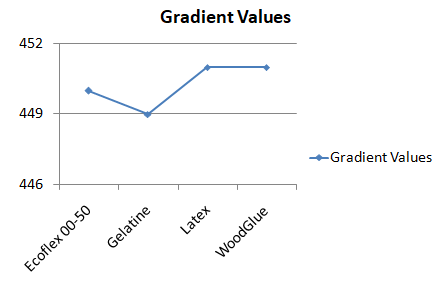
\includegraphics[scale=0.8]{Gradient.PNG}   
\caption{Sample visualization / Experimental gradient value}
\label{fig:sample_grad}
\end{figure}

% Note: Replace with your actual screenshot images when available
% \begin{figure}[htbp]
% \centering
% \includegraphics[width=0.8\textwidth]{liveimg.png}   
% \caption{Live fingerprint image from testing dataset}
% \label{fig:live_img}
% \end{figure}

\chapter{Sample Code}
\section*{Evaluation and Feature Extraction Script}

% Include code/text in verbatim environment to display exactly as written
\begin{verbatim}  
close all;
clear;
clc;

% 1. Read input image file
[filename, pathname] = uigetfile('*.png', 'Select an image', 'Dataset\Testing');
I = imread(fullfile(pathname, filename));
addpath('Waveatom');
val = wave(I);

% 2. Extract minutiae features
[rgbImage, ridge_xy, bifurcation_xy] = minutiaeextract(val);

% 3. Model prediction
if cnnPredict == 1
    uiwait(msgbox(sprintf('LIVE'), 'RESULT'));
else
    uiwait(msgbox(sprintf('FAKE'), 'RESULT'));
end
\end{verbatim}

\section*{Feature Extraction for Dataset Materials}
\begin{verbatim}
clc;
clear;

load fpsFs;
FList = ReadImageNames('DataSet');
Index = contains(FList, 'Testing\Fake\Ecoflex 00-50');
TestF_name_G = FList(Index, :);
TestF_G = fpsFs(Index, :);

net = trainSoftmaxLayer(TrainF', Ts);
[~, cnn_predict] = max(net(TestF'));
cp = classperf(TestL, cnn_predict);
\end{verbatim}
